\documentclass[tikz,border=3pt]{standalone}
\usepackage[utf8]{inputenc}
\usepackage[T1]{fontenc}
\usepackage{lmodern}
\renewcommand{\familydefault}{\sfdefault}
\usepackage{sansmath}\sansmath
\usepackage{chemfig}
\usepackage{pgfplots}\pgfplotsset{compat=1.18,/pgf/number format/use comma,/pgf/number format/1000 sep={.}}
\usetikzlibrary{arrows.meta,calc,positioning,decorations.pathmorphing,patterns}
% paleta del sitio
\definecolor{nar}{HTML}{E8680C}\definecolor{narc}{HTML}{FFB35C}\definecolor{hielo}{HTML}{FFF3E8}
\definecolor{tinta}{HTML}{1D1D1F}\definecolor{gris}{HTML}{6E6E73}\definecolor{lila}{HTML}{7C5CF0}
\definecolor{azul}{HTML}{2F6FD6}\definecolor{menta}{HTML}{17A673}\definecolor{coral}{HTML}{E8342A}
\begin{document}
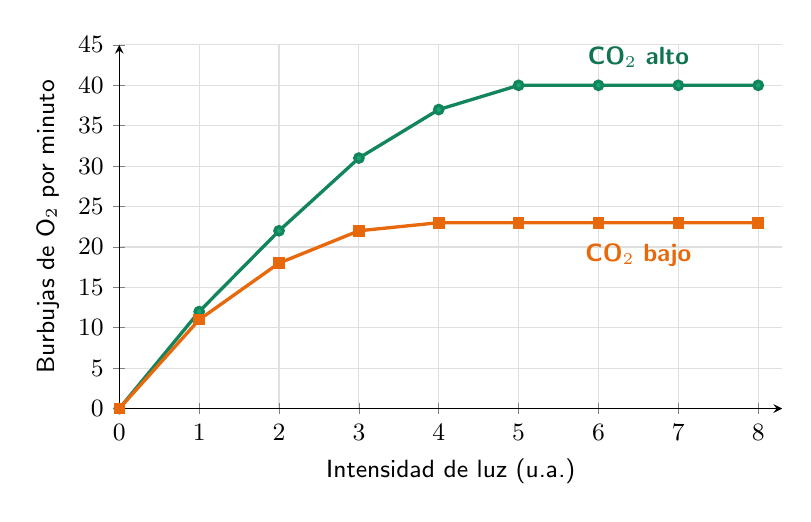
\begin{tikzpicture}[font=\small]
\begin{axis}[width=10cm,height=6.2cm,axis lines=left,xmin=0,xmax=8.3,ymin=0,ymax=45,xtick={0,1,...,8},ytick={0,5,...,45},
  grid=major,grid style={gray!25},xlabel={Intensidad de luz (u.a.)},ylabel={Burbujas de O$_2$ por minuto},clip=false]
\addplot[menta!80!black,very thick,mark=*,mark options={fill=menta,scale=0.75}] coordinates {(0,0)(1,12)(2,22)(3,31)(4,37)(5,40)(6,40)(7,40)(8,40)};
\addplot[nar,very thick,mark=square*,mark options={fill=nar,scale=0.75}] coordinates {(0,0)(1,11)(2,18)(3,22)(4,23)(5,23)(6,23)(7,23)(8,23)};
\node[menta!70!black,font=\small\bfseries,anchor=south] at (axis cs:6.5,41) {CO$_2$ alto};
\node[nar,font=\small\bfseries,anchor=north] at (axis cs:6.5,21.5) {CO$_2$ bajo};
\end{axis}
\end{tikzpicture}
\end{document}
